%5.1	Descripción de la implementación 
%Describir cómo el proyecto se divide en etapas. Presentar detalle de las etapas.
\section{Implementation Review}
The implementation was separated in three large stages. The first one was the development of a test application which runs in Mac OS X and was developed using C++ and OpenFrameworks. The second stage consisted of the development of particular concept tests, regarding some possible technical difficulties I expected to have. The third stage was the actual development of the final application.

\subsection{First Stage Report}
The text below is extracted as it was delivered to Frédéric and Tiberio at the end of the first stage. Keep this in mind while reading.

\subsubsection{Process}
The first part of my stance in Chalon was spent in training myself in C++. Although I've used it for some college assignments before I wasn't in the shape of starting a new project. I made a pair of experiments to get used to the differences between C++ and the languages I already used. This period took place from the monday january 14 to the friday january 25.

The second part of my stance was concerned with a quick prototype implementation of the 3D Annotation System. This prototype would run in a regular PC providing the basic functionality expected from the final system, but whose user interaction requirements where simplified in the sake of simplicity. As of tuesday, march 24 the prototype was able to load a .3DS model, display it with textures and topological information and allow the user to select vertices. This day took place a meeting with Frédéric and Sebastian to evaluate and comment the prototype and choose the direction of the next steps to take. Strictly speaking this part of the process is over, although I'll end the prototype with the planned requirements.

The calendar so far looks like this:

\begin{center}
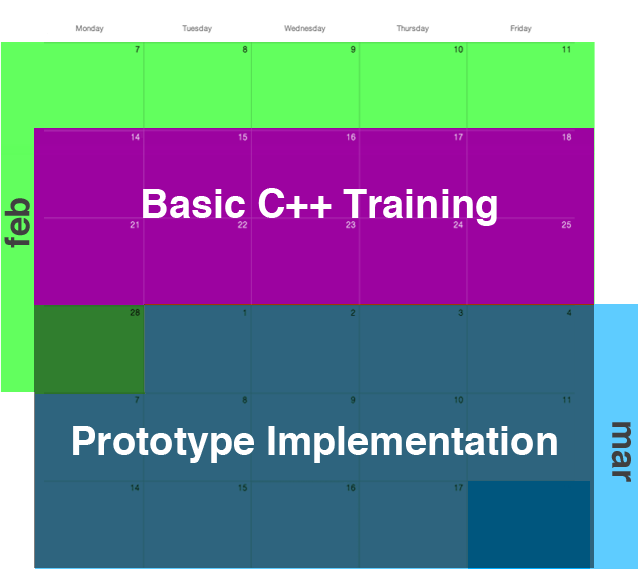
\includegraphics[scale=0.5]{Images/first_calendar.png}
\end{center}
\subsubsection{Prototype}

\hspace{6mm}{\large Requirements:}

Loads multi-meshed and textured 3DS models.
Displays the textured model.
Displays on the top of the model its topological information (vertices and edges).
Allows the user to select a set of vertices using the mouse.
Allows the user to add an annotation using the keyboard.
Retrieves the annotations attached to the selected vertices.
The requirements in italics are those which weren't fulfilled before the meeting.\\



{\large Tech specs:}

The prototype was developed on Mac OS X 10.6, using XCode 3.2.4 as IDE and OpenFrameworks as an entry level framework which simplifies some of the tasks needed to fulfill the requirements. Most of the work on the prototype was made on the top of the ofx3DModelLoader OpenFrameworks add-on version.\\

{\large Design decisions:}

The selection of OpenFrameworks as the general purpose framework of the project modeled some of the decisions toked. The selection of ofx3DModelLoader as the base of the code to load and display defined that the archive type to load was 3Ds. My prior use of the Color Picking to select objects in 3D space through a 2D interface made it the best option to me at the time. The selection of vertices as the basic anchor of the annotations was made thinking about vertices as the basic element of any 3D object.

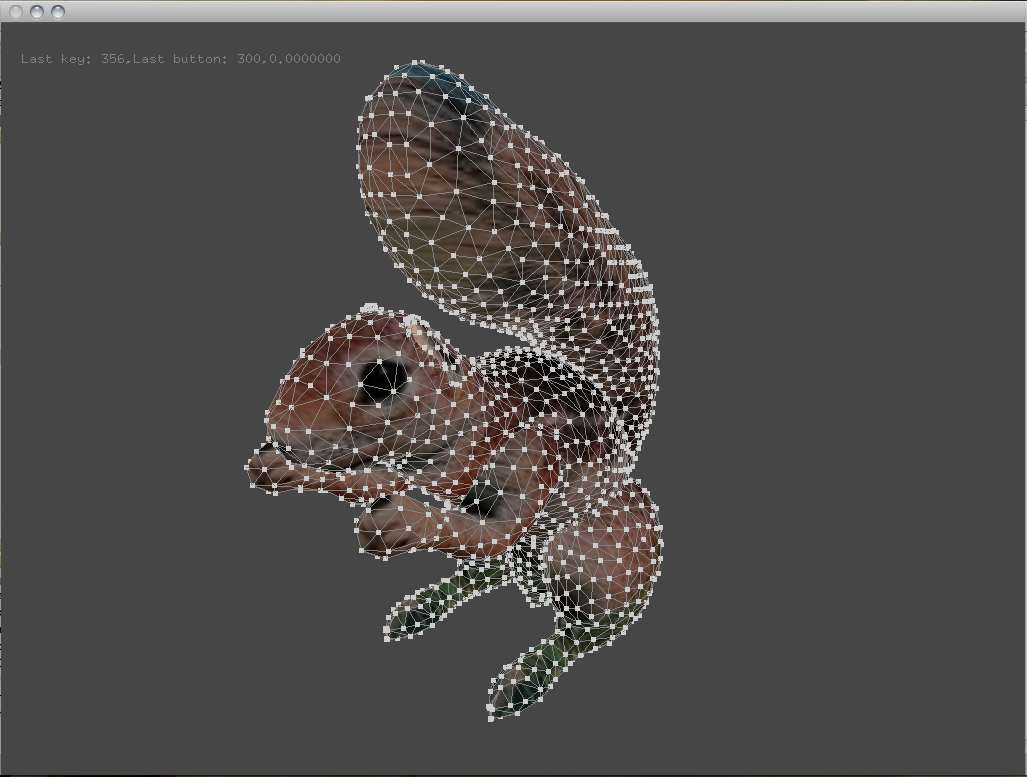
\includegraphics[scale=0.18]{Images/prototype1_normal.png}
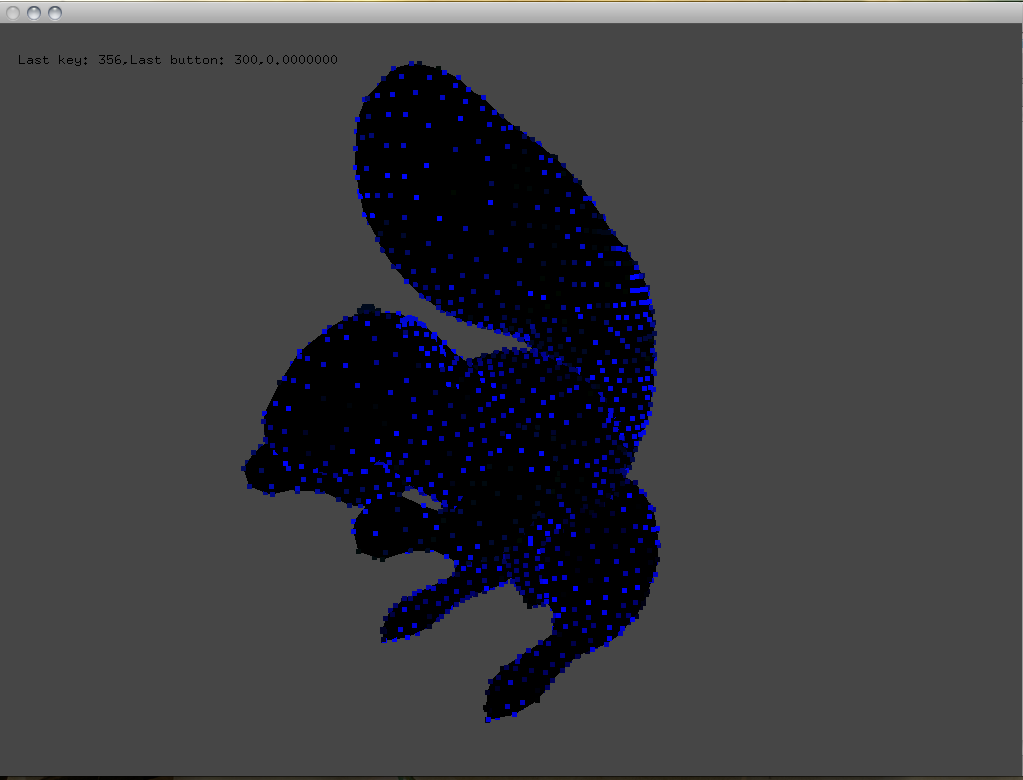
\includegraphics[scale=0.18]{Images/prototype1_picking.png}

\subsubsection{Conclusions}
\begin{enumerate}
	\item The selection of Color Picking wasn't the best, it took me most of the time of the development of the prototype (because of unseen difficulties) and isn't suitable to use in following versions of the product, given the user interaction requirements\footnote{I thought that at that point of the development, it turned that with the use of the tablet the color picking algorithm is not only suitable but presents meaningful advantages.}.
	\item The selection of vertices as the anchor points of the annotations was changed during the meeting. Although it's true that the vertices are the basic element of any 3D model, the polygons are a more natural and meaningful part to attach annotations to.
	\item Another meaningful decision took from the first prototype was the selection of OpenSceneGraph and not Openframeworks as a more suitable framework to base the work on.
	\item A talk with Tiberio exposed the need to evaluate the user interaction with the system before building the complete product. Somewhat like a prior iteration on the UX design. It's also needed to make a more formal definition of an annotation \footnote{A sudden cut in the expected development time rendered this impossible.}.
	\item During the meeting with Frédéric and Sebastian, Frédéric pointed the possibility of using speech recognition to make the annotations as a more natural way to interact with the system (vs the option thought before, of using an Android powered tablet to write down the annotations)\footnote{The reasons behind not following this alternative have been already discussed in the previous chapter.}.
\end{enumerate}

\subsection{Second Stage}
This period took place from the star of April to the second week of May. Definitively not my most productive time in Chalon, nevertheless I think it was a necessary period of time\footnote{However, it could last a little less.}. During the second stage I was deeply concerned about my inexperience with the tools used, so I experimented and tried tutorials in order to gain experience. I was familiar with the Android platform, the Java programming language and the Eclipse IDE, nevertheless I felt I should try to make some stuff before starting to work in the project. This way I could avoid beginner errors on the application. Those tests are not related to the subject of this document in any other way than the acquisition of technical abilities to proceed in the implementation of the project. I also used a code example made by Sébastien to display and navigate 3D scenes in the cave.

At the end of the second stage I was given the code made by Philippe that addressed similar objectives as this project.

\subsection{Third Stage}
The third stage begun with the design and programming of the tablet's software. I had a hard time trying to connect the tablet to a WiFi router provided by the Institute's Network Administrator. I decided to buy my own router and start experimenting with video streaming to the tablet, it took me nearly a week to make it work correctly. Another issue that took me more time than I expected was the programming of the 3D Joysticks. 

After some time tweaking the tablet app and the scene streaming a progress meeting was made with Frédéric and Sébastien. After this meeting I had only one week left to implement the parts of the software I avoided during most of the time. I worked hard that last week and ended with a complete solution, and almost the proposed one. As I've already commented, the difference between the application delivered and the one designed is that the delivered application is incapable of create and display the comments as marquees. So the user, to review the annotations must go to the list in the tablet app, and review one by one.